\chapter[Development of methods to complement metagenomic analysis of Ace Lake]{Development of quantitative epifluorescence microscopy and metaproteomic methods to complement metagenomic analysis of Ace Lake}
\label{ch:ace}
\acresetall

%-----------------------------------------------------------------------------------------------
\section*{Co-authorship statement}
\addcontentsline{toc}{section}{Co-authorship statement}

Sections from this chapter~\ref{ch:ace} have been published as:\\

Federico M. Lauro, Matthew Z. DeMaere, \textbf{Sheree Yau}, Mark V. Brown, Charmaine Ng,
David Wilkins, Mark J. Raftery, John A.E. Gibson, Cynthia Andrews-Pfannkoch, Matthew Lewis,
Jeffery M. Hoffman,Torsten Thomas, and Ricardo Cavicchioli. 
An integrative study of a meromictic lake ecosystem in Antarctica.
\emph{\underline{International Society of }}
\emph{\underline{Microbial Ecology Journal}}
5:879--895, 2011.\\

I performed the metaproteomic mass spectra analysis, epifluorescence imaging,
microbial and viral counts and wrote the corresponding sections of the publication.
Only these parts of the publication are included in the results and discussion of this chapter.

Analyses performed by others that support the work presented in this chapter are as follows:
Research was designed by Federico Lauro, Mark Brown, Torsten Thomas, John Gibson and Ricardo Cavicchioli.
Sample collection was performed by Federico Lauro, Mark Brown, Torsten Thomas, Jeffery Hoffman and Ricardo Cavicchioli.
\textsc{DNA} extraction and clone library preparation of 2006 samples was performed by Cynthia Andrews-Pfannkoch and Jeffery Hoffman of the \ac{JCVI}.
\textsc{DNA} sequencing quality control was performed by Matthew Lewis of the \ac{JCVI}.
Metagenomic sequence filtering, mosaic assembly and annotation was performed by Matthew DeMaere.
Protein extraction, one-dimensional sodium dodecyl sulphate-polyacrylamide gel electrophoresis and liquid chromatography mass spectrometry performed by Charmaine Ng.
Assistance in mass spectra analysis was provided by Mark Raftery.
\newpage

%----------------------------------------------------------------------------------------------
\section{Abstract}



%---------------------------------------------------------------------------------------------
\section{Introduction}
Ace Lake is a meromictic saline lake in the Vestfold Hills, Antarctica. 
It is the best studied of all the meromictic lakes in the Vestfold Hills and possibly Antarctica.
Extensive physical, chemical and biological data has been collected from Ace Lake in the last decades \cite{Rankin1999}.
%This is summarised in the figure of the whole lake. %figure of lake.
However, the microbial community has largely been probed using culture-based or phenotypic means, or inferred from the lake's geochemistry.
An analysis of the 16S \ac{SSU} diversity was completed of the sediment showed microbial diversity was reduced \cite{Bowman2000a}.
%What else? about the diversity from Bowman paper? Link to the intro.

Ace Lake is a highly stratified lake system, 25 m deep at its deepest point.
It is ice-covered for approximately 9 months of the year and thaws some summers. %check
Water is marine-derived and a largely neutral water balance has ensured salinity is close to that of seawater.
Although a lens of fresher water from melted surface ice can be generated in the summer months, this only mixes when the lake is ice-free and not to great depth \cite{Rankin1999}.
The lake is physically separated into an aerobic mixolimnion, a steep chemocline/oxycline at 12.7 m and an anoxic monimolimnion below.
The monimolimnion is sulfidic and methanogenic; both compounds have presumably accumulated through activity from \ac{SRB} and methanogenic archaea respectively.

As a physically and chemically well-characterised system of moderate diversity, Ace Lake was chosen as a model ecosystem to implement an integrated metagenomic and metaproteomic analysis.
Combining both approaches would allow assessment of the metabolic potential of the system and identify the active members of the community and processes at time of sampling.
In other words, discern who's there?, what could they be doing? and are they really doing it?
Samples were obtained down the depth profile at 5, 11.5, 12.7, 18 and 23 m depths corresponding to each of the three zones.
Sampling was conducted as part of the \ac{GOS} expedition \cite{Rusch2007} by using size fractionation of microbial biomass onto 3.0, 0.8 and 0.1 \textmu{}m membrane filters.
%consider leaving above line out.

Microbial and viral community composition was assessed from the metagenomic dataset.
Significant differences were found in taxonomic composition of each size fraction within each sample depth and stratification of the microbial community between the three zones of Ace Lake.
The mixolimnion community is similar to a marine surface water assemblage consisting of a high abundance of the SAR11 clade of \emph{Alphaproteobacteria} related to ``\emph{Candidatus} Pelagibacter ubique'' and green algae of the order \emph{Mamiellales}.
However, diversity is reduced by one order of magnitude reduced \cite{Lauro2011}.
Unlike Southern Ocean surface water, the mixolimnion is overrepresented in \emph{Cyanobacteria} related to \emph{Synechococcus} and \emph{Actinobacteria}, which may represent taxa that mark the transition of a marine to lake community.
A dense, near clonal population of \acl{GSB} related to \emph{Chlorobium} termed C-ace reside at the chemo/oxycline at 12.7 m \cite{Ng2010a, Lauro2011}.
Below, in the anoxic monimolimnion is a diverse, primarily heterotrophic community with abundant \ac{SRB} and methanogenic \emph{Archaea}.
%How abundant were the methanogens??

Preliminary work on the metaproteome down the vertical profile of Ace Lake has been performed using the \ac{NCBI} \ac{NR} database \cite{Ng2010b}.
However, there were few protein identifications were achieved using the unmatched genomic database \cite{Ng2010b}.
%Put in a table of the rates of matches...
Identification rate reduced as diversity of the sample increased.
A focused metaproteogeonomic analysis conducted on the dense \ac{GSB} layer using the matched metagenome as the database resulted in many more protein identifications compared to using the \ac{NR} database \cite{Ng2010b}.
Assessment of the genetic complement of Ace Lake showed a concurrent stratification of the functional potential in each zone of Ace Lake \cite{Lauro2011}.
Significantly, \ac{GSB} appeared to be crucial in the lake ecosystem as they had the greatest genetic potential for nitrogen and carbon fixation as well as sulphur cycling\cite{Ng2010b, Lauro2011}.
Metaproteomic analysis was able to identify which proteins were actively expressed and thus the active pathways of the \ac{GSB} metabolism which are so crucial to the function of the lake \cite{Ng2010a}.

This study aimed to expand on the metagenomic analysis of the water column of Ace Lake using complementary analyses.
Metaproteomic analysis was used to identify expressed proteins of the 0.1 \textmu{}m size fraction Ace Lake using a matched metagenomic databases for protein identification to infer which taxa and metabolic processes were active at time of sampling.
To determine cellular and viral densities and validate the efficacy of size-fractionation with a modified epifluorescence microscopy procedure was developed and implemented.

%---------------------------------------------------------------------------------------------

\section{Materials and methods}
\label{sec:ace_mm}
\subsection{Ace Lake samples}
Water samples were collected from Ace Lake (68$^{\circ}$28$'$23.2$''$S, 78$^{\circ}$11$'$20.8$''$E), Vestfold Hills, Antarctica on 21 and 22 December 2006. 
A 2 m hole positioned above the deepest point (25 m depth) of the lake was drilled through the ice cover of Ace Lake to reach the lake surface.
A volume of 1--10 L was collected by sequential size fractionation through a 20 \textmu{}m pre-filter directly onto filters 3.0, 0.8 and 0.1 \textmu{}m pore-sized, 293 mm polyethersulfone membrane filters (Rusch et al., 2007), along the depth profile as described previously \cite{Ng2010a}.
Samples were taken in the order, 23, 18, 14, 12.7, 5 and finally, 11.5 m.

After samples from each depth were collected, the sample racks were sequentially washed with 2 $\times$ 25 L 0.1 N NaOH, 2 $\times$ 25 L 0.053\% NaOCl, and 2 $\times$ 25 L fresh water. 
The sample hose was flushed with water from each depth before being applied to the filters. 
A \emph{Chlorobium} signature was identified at 5 m, but not immediately above the \ac{GSB} layer at 11.5 m. 
As the next sample taken after sampling at 12.7 m was at 5 m, and then 11.5 m, despite all equipment being thoroughly washed with bleach, NaOH and water, 
the simplest explanation for the \ac{GSB} signature at 5 m is carry-over from sampling of the dense biomass at 12.7 m. 

A sonde probe (\textsc{YSI} model 6600, \textsc{YSI} Inc., Yellow Springs, \textsc{OH}, \textsc{USA}) was used to record depth, dissolved oxygen content, pH, salinity, temperature and turbidity throughout the water column of the lake. 
Total organic carbon was determined using a total organic carbon analyzer, TOC-5000A (Shimadzu, Kyoto, Japan) equipped with a \textsc{ASI}-5000A auto sampler (Shimadzu), and particulate organic carbon by standard protocols 
\url{(http://www.epa.gov/glnpo/lmmb/methods/about.html)} 
at the Centre for Water and Waste Technology, \textsc{UNSW}.

\subsection{\textsc{DNA} sequencing and data cleanup}
\textsc{DNA} extraction and Sanger sequencing was performed on 3730xl capillary sequencers (Applied Biosystems, Carlsbad, \textsc{CA}, \textsc{USA}) and pyrosequencing on \textsc{GS20 FLX} Titanium (Roche, Branford, \textsc{CT}, \textsc{USA}) at the \acl{JCVI} in Rockville, \textsc{MD}, \textsc{USA} \cite{Rusch2007}. 
The scaffolds and annotations will be available via \ac{CAMERA} and public sequence repositories such as the \ac{NCBI} and the reads will be available via the \ac{NCBI} Trace Archive. 

Sanger reads were trimmed according to quality clear ranges.
The quality of pyrosequencing reads was assessed as follows: 
a \ac{BLAST} nucleotide database was created from the Sanger reads of the 0.1 \textmu{}m fraction of samples GS230, GS231 and GS232 (see Table of metagenomic data). %%Add link to table of metagenomic data. Change sample IDs to depths?
After blasting the corresponding pyrosequencing reads against each database with a minimum bitscore of 80 and maximum e-value of 0.1, reads were binned according to length.
The percentage of reads for each bin lacking a match to the Sanger read database was recorded. 
The percentage reads at least 25\% repetitive after \textsc{MDUST} \cite{Morgulis2006} analysis at default settings, and the percentage of reads containing N's, were assessed. 
In contrast to earlier pyrosequencers \cite{Huse2007}, no length-dependent bias in reads containing N's was observed. 
However, short reads had a disproportionately high number of repeats. 
Moreover, based on the proportion of reads with no match to the Sanger data set, both very short and very long reads had a disproportionately high number of errors; an observation that was previously reported \cite{Huse2007}.

On the basis of this analysis, a three step filtering process was applied to each sample. 
Reads were initially run through the Celera \textsc{sffToCA} \cite{Miller2008} pre-processor followed by \textsc{Lucy} \cite{Chou2001} and finally, excluding the bottom 8\% and top 3\% of reads determined from the read length distribution. 
As the \textsc{sffToCA} (v5.3) pre-processor removes all reads with a perfect prefix of any other read it overcomes the `perfect duplicates’ problem \cite{Gomez-Alvarez2009}.
 
After this process, $<$5\% of the reads belonged to clusters of duplicates with three or more reads, and \ac{COG} of proteins classification of these reads showed an over-representation of category L (replication, recombination and repair) that includes mobile genetic elements, which are often duplicated, suggesting a potential biological significance for the duplicated reads. 
It is possible these residual duplications are a result of high gene copy number or localized fragility of DNA sequences that might be biasing the shear points.

\subsection{Metagenomic DNA assembly and annotation}
Mosaic assemblies were generated for each sample fraction using Celera \ac{WGS} Assembler v5.3 \cite{Myers2000}. 
For each assembly, the runtime parameters used were as outlined for 454 sequencing data in the published standard operating procedure\\ 
\url{(http://sourceforge.net/apps/mediawiki/wgs-assembler/index.php?title 1⁄4SFF\_SOP)}. 
As none of the samples can be considered clonal, these are regarded as stringent assemblies \cite{Rusch2007}. 
Each 0.1 \textmu{}m fraction assembly was a hybrid of Sanger and 454 read data, wherein the estimated genome size was manually set to minimize the number of unitigs from abundant organisms being falsely classified as degenerate \cite{Rusch2007}. 
Annotation of each sample fraction assembly was carried out using an in-house pipeline, wherein the pipeline stages consisted of genomic feature detection and subsequent annotation. 
Detected features consisted of \acp{ORF}, transfer \textsc{RNA} and \ac{rRNA}. 
Each detected \ac{ORF} was further annotated by \ac{BLAST} comparison against \ac{NR}, Swissprot and \ac{KEGG}-peptide sequence databases and by \ac{HMMER} comparison against \ac{TIGRFAM} \cite{Haft2001}, \ac{COG} \cite{Tatusov1997, Tatusov2003} and known marker genes \cite{vonMering2007}.
In all cases the cut-off e-value was a maximum of 1e$-$5. 


\subsection{Epifluorescence microscopy}
Samples of unfiltered lake water and the flow-through from 3.0 and 0.8 \textmu{}m filters from all depths were collected on November 2008 and fixed on site in formalin 1\% (v/v). 
The samples were stored at $-$80$^{\circ}$C for subsequent direct counts of cells and \acp{VLP}. 
Enumeration was performed according to the method of \citet{Patel2007} with modifications. 
%desribe the set up of the filter apparatus!
Lake water samples were filtered onto 0.01 \textmu{}m pore-size polycarbonate filters (25 mm Poretics, \textsc{GE} Osmonics, Minnetonka, \textsc{MN}, \textsc{USA}). 
Filters were air dried, then placed with the back of the filter on top of a 30 ml aliquot of 0.1\% (w/v) molten low-gelling-point agarose and allowed to dry at 30$^{\circ}$C. 
Samples were stained by the addition of 1 ml working solution (1 in 400 dilution in 0.02 \textmu{}m filtered sterile Milli-Q) of \textsc{SYBR} Gold$^{\textregistered}$ (Molecular Probes, Eugene, \textsc{OR}, \textsc{USA}) to 25 ml of mounting medium (\textsc{VECTASHIELD} HardSet, Vector Laboratories, Burlingame, \textsc{CA}, \textsc{USA}). 
Stained samples were counted immediately, or stored at $-$20$^{\circ}$C for up to a week before counting. 
Samples were visualised under wide-blue filter set (excitation 460--495 nm, emission 510--550 nm) with an epifluorescence microscope (Olympus BX61, Hamburg, Germany).


\subsection{Metaproteomic analysis}
Proteins were extracted from membrane filters from all 0.1 \textmu{}m fractions from the six depths (5, 11.5, 12.7, 14, 18 and 23 m), and \ac{1D-SDS PAGE} and in gel trypsin digestion, liquid chromatography and mass \ac{MS}, and \ac{MS-MS} data analysis and validation of protein identifications performed as previously described \cite{Ng2010a}, with minor modifications.
The specta generated were searched against the protein sequence database corresponding to that depth constructed from the 0.1 \textmu{}m mosaic assemblies. 
The number of protein sequences in each database were as follows: 5 m, 138,208; 11.5 m, 133,948; 12.7 m, 27,142; 14 m, 62,436; 18 m, 71,512; and 23 m, 128,878. 
Scaffold (version Scaffold\_2\_05\_01, Proteome Software Inc., Portland, \textsc{OR}, \textsc{USA}) was used to validate \ac{MS-MS}-based peptide and protein identifications. 
Peptide and protein identifications were accepted if they could be established at $>$95\% and 99\% probability, respectively, as specified by the Peptide Prophet algorithm \cite{Keller2002}. 
Protein identifications required the identification of at least two peptides.
 
Proteins that contained similar peptides and could not be differentiated based on \ac{MS-MS} analysis alone were grouped to satisfy the principles of parsimony and are referred to as a protein group. 
Spectral counting was used to semi-quantitively estimate protein abundance. 
The total assigned spectra that matched to each identified protein were exported from \textsc{Scaffold} 2.0. 
For similar proteins that have shared peptides (a protein ambiguity group), spectra were assigned to the protein with the most unique spectra. 
To normalise for variation in total spectra acquired between sample replicates, the number of spectra of each protein was multiplied by the average total spectra divided by the total spectra of the individual replicate. 
The spectral count of each protein was averaged across the replicates. 
As longer proteins are more likely to be detected, the average spectral counts were divided by the length of the protein. 
This value is equivalent to the normalised spectral abundance factor \cite{Florens2006, Zybailov2006}. 
In order to compare the relative abundance of proteins between depths, the normalised spectral abundance factor was divided by the average read depth of the contig (scaffold or degenerate) to which the protein mapped. 

If $>$90\% of a scaffold’s length consisted of surrogate (highly degenerate unitig) sequence, the average read depth of the surrogate was used. 
For identified proteins that were part of a protein group the longest protein length and largest read depth value in the group was used. 
Pairwise comparisons of each zone were conducted on \ac{COG} assigned proteins. 
The normalised spectral counts from each protein was aggregated based on their \ac{COG} annotation. 
All proteins that were part of an ambiguity group were confirmed to share the same \ac{COG} annotation to ensure counts were not biased because of the common spectra.

The summed spectral counts from 5 and 11.5 m (mixolimnion), and 14, 18 and 23 m (monimolimnion) were pooled. 
Statistical significance of differences between each zone was assessed using Fisher's exact test, with confidence intervals at 99\% significance calculated by the Newcombe–Wilson method and Holm-Bonferroni correction (P-value cutoff of 1e$-$5) in \ac{STAMP} \cite{Parks2010}. 
All proteins identified, including their gene identifier, normalised spectral abundance, \ac{COG} and \ac{KEGG} Orthology identifiers, \ac{KEGG} locus tag and matching \ac{COG} or \ac{KEGG} description are provided in Supplementary Table S1.



%---------------------------------------------------------------------------------------------

\section{Results and discussion}

\subsection[Epifluorescence microscopy methodology]{Development of epifluorescence microscopy methodology for cell and \acp{VLP} enumeration}
As part of the integrative study of Ace Lake, an epifluorescence microscopy methodology was developed.
Motivation for visualising microbiota from size fractionated water samples was twofold. 
Firstly, visualising microbiota from water samples allows examination of cellular morphologies and more importantly, enumeration of cells and \acp{VLP}.
Absolute cellular and \ac{VLP} densities are not easily inferred from the metagenomic data and necessitates a complementary method of determination.
Determining viral densities is extremely important as the first studies to do so found that viruses are the most numerous biological entities on the planet and likely play a large role in plankton mortality in the ocean \cite{Bergh1989,Proctor1990}. %Why is determining cellular densities important
\ac{VLP} counts from marine environments vary with depth and trophic status ranging from 10$^6$ to 10$^8$ \acs{VLP} ml$^{-1}$ \cite{Suttle2005}. %cite Fuhrman review paper too.
Viral counts from various aquatic environments have differed from site to site indicating a variable role of virally mediated mortality. %ref microbial ecology of the oceans.%cite Fuhrman review.

Secondly, size fractionation of suspended microbial biomass from aquatic environments has been utilised as part of the landmark Sargasso Sea metagenomic study \cite{Venter2004} and subsequent \ac{GOS} expedition \cite{Rusch2007}.
The Ace Lake samples were collected using the same sampling strategy as the \ac{GOS} dataset but has sequence information from all three filter sizes. 
Thus, the visualisation of microbial morphologies from each stage of the filtration process would allow validation of the filtration process.

Developing a revised method for the simultaneous counts of cells and \acp{VLP} was necessary due to inability to source 25 mm diameter 0.02 \textmu{}m pore-size Anodisc filters (Whatman) that have been long used with fluorescent nucleic acid dyes for this purpose \cite{Hennes1995, Noble1998}. 
They were marked for discontinuation in December 2008 after the take over of Whatman by \textsc{GE} Healthcare and was the cause of a global shortage that was strongly opposed by the viral ecology community \cite{Torrice2009}.
Since conducting this research, production of 25 mm Anodisc filters has resumed after the petitioning of \textsc{GE} Healthcare by the environmental virology community. 
Cost of Anodiscs filters are relatively higher than they were previously. %%%Check!
Nonetheless, the need for alternative methodolodies during the shortage was so great that alternative protocols were developed independently in other research groups \cite{Budinoff2011, Diemer2012} stressing the importance of an affordable method of direct viral counts and the utility of alternative methodologies. %Look up that poster with beads direct on slide.

Clear \ac{PCTE} filters were selected for use as a viable alternative product for the following reasons. 
\begin{enumerate}
\item They have defined pore-size. %Look up track etch technology
\item They are available in 0.015 \textmu{}m pore-size allowing capture of \acp{VLP}.
\item They have previously been used for \acp{VLP} enumeration \cite{Hara1991, Proctor1992}.
\item They have a long history of use with cellular enumeration \cite{Hobbie1977} and can therefore be easily adopted for widespread use.
\end{enumerate}

%get refs for hara1991 and Proctor1992.

There are several disadvantages to using \ac{PCTE} membranes over Anodiscs which are as follows.
\begin{enumerate}
\item Polycarbonate is not as robust as 25 mm diameter Anodisc filters that have a built in plastic support ring around the edge.
\item The polycarbonate of \ac{PCTE} filters cannot be blotted dry as the Al$_{2}$O$_{e}$ of Anodisc filters.
\item \ac{PCTE} filters appear to have high background fluorescence. %ref
\item \ac{PCTE} filters have a much slower flow rate that Anodisc filters. %ref.
\end{enumerate}

The protocol used is detailled in the materials and methods \ref{sec:ace_mm}.
The main disadvantages of using \ac{PCTE} were overcome for the purposes required for this study.
To counteract the fragility of the \ac{PCTE} filters, vacuum filtration was not performed above X pressure limit and filters.
No cracks or tears were observed during visualisation.
\ac{PCTE} filters also have a tendency to crinkle when mounted on the glass slide making visualisation of cells and \acp{VLP} on a single focal plane difficult.
Agarose was used to embed the filters to help flatten the membrane and aid in mounting.
However, this was not strictly necessary if filters were dried well and the membrane mounted carefully so that it was pressed flat against the glass slide.
The back ground fluorescence of the clear filters was low when stain is only incorporated into the mountant after filtration rather than staining in the column before filtration.

Filtration onto very small pore-size also necessitated a very strong seal of the filter column against the glass, but the slow flow-rate was not a property of the \ac{PCTE} filters that could be overcome.
As the filtration and visualisation was performed on fixed samples in the laboratory rather than in the field, the time taken for filtration of 2--3 hours for each sample, this was not deemed problematic for this study.


Overall, a viable alternative methodology was successfully developed for visualisation and enumeration of cells and \acp{VLP} using \ac{PCTE} membrane filters was successful and could be used as an alternative to Anodisc-filters \figref{fig:ace_microscopy}.
\begin{figure}
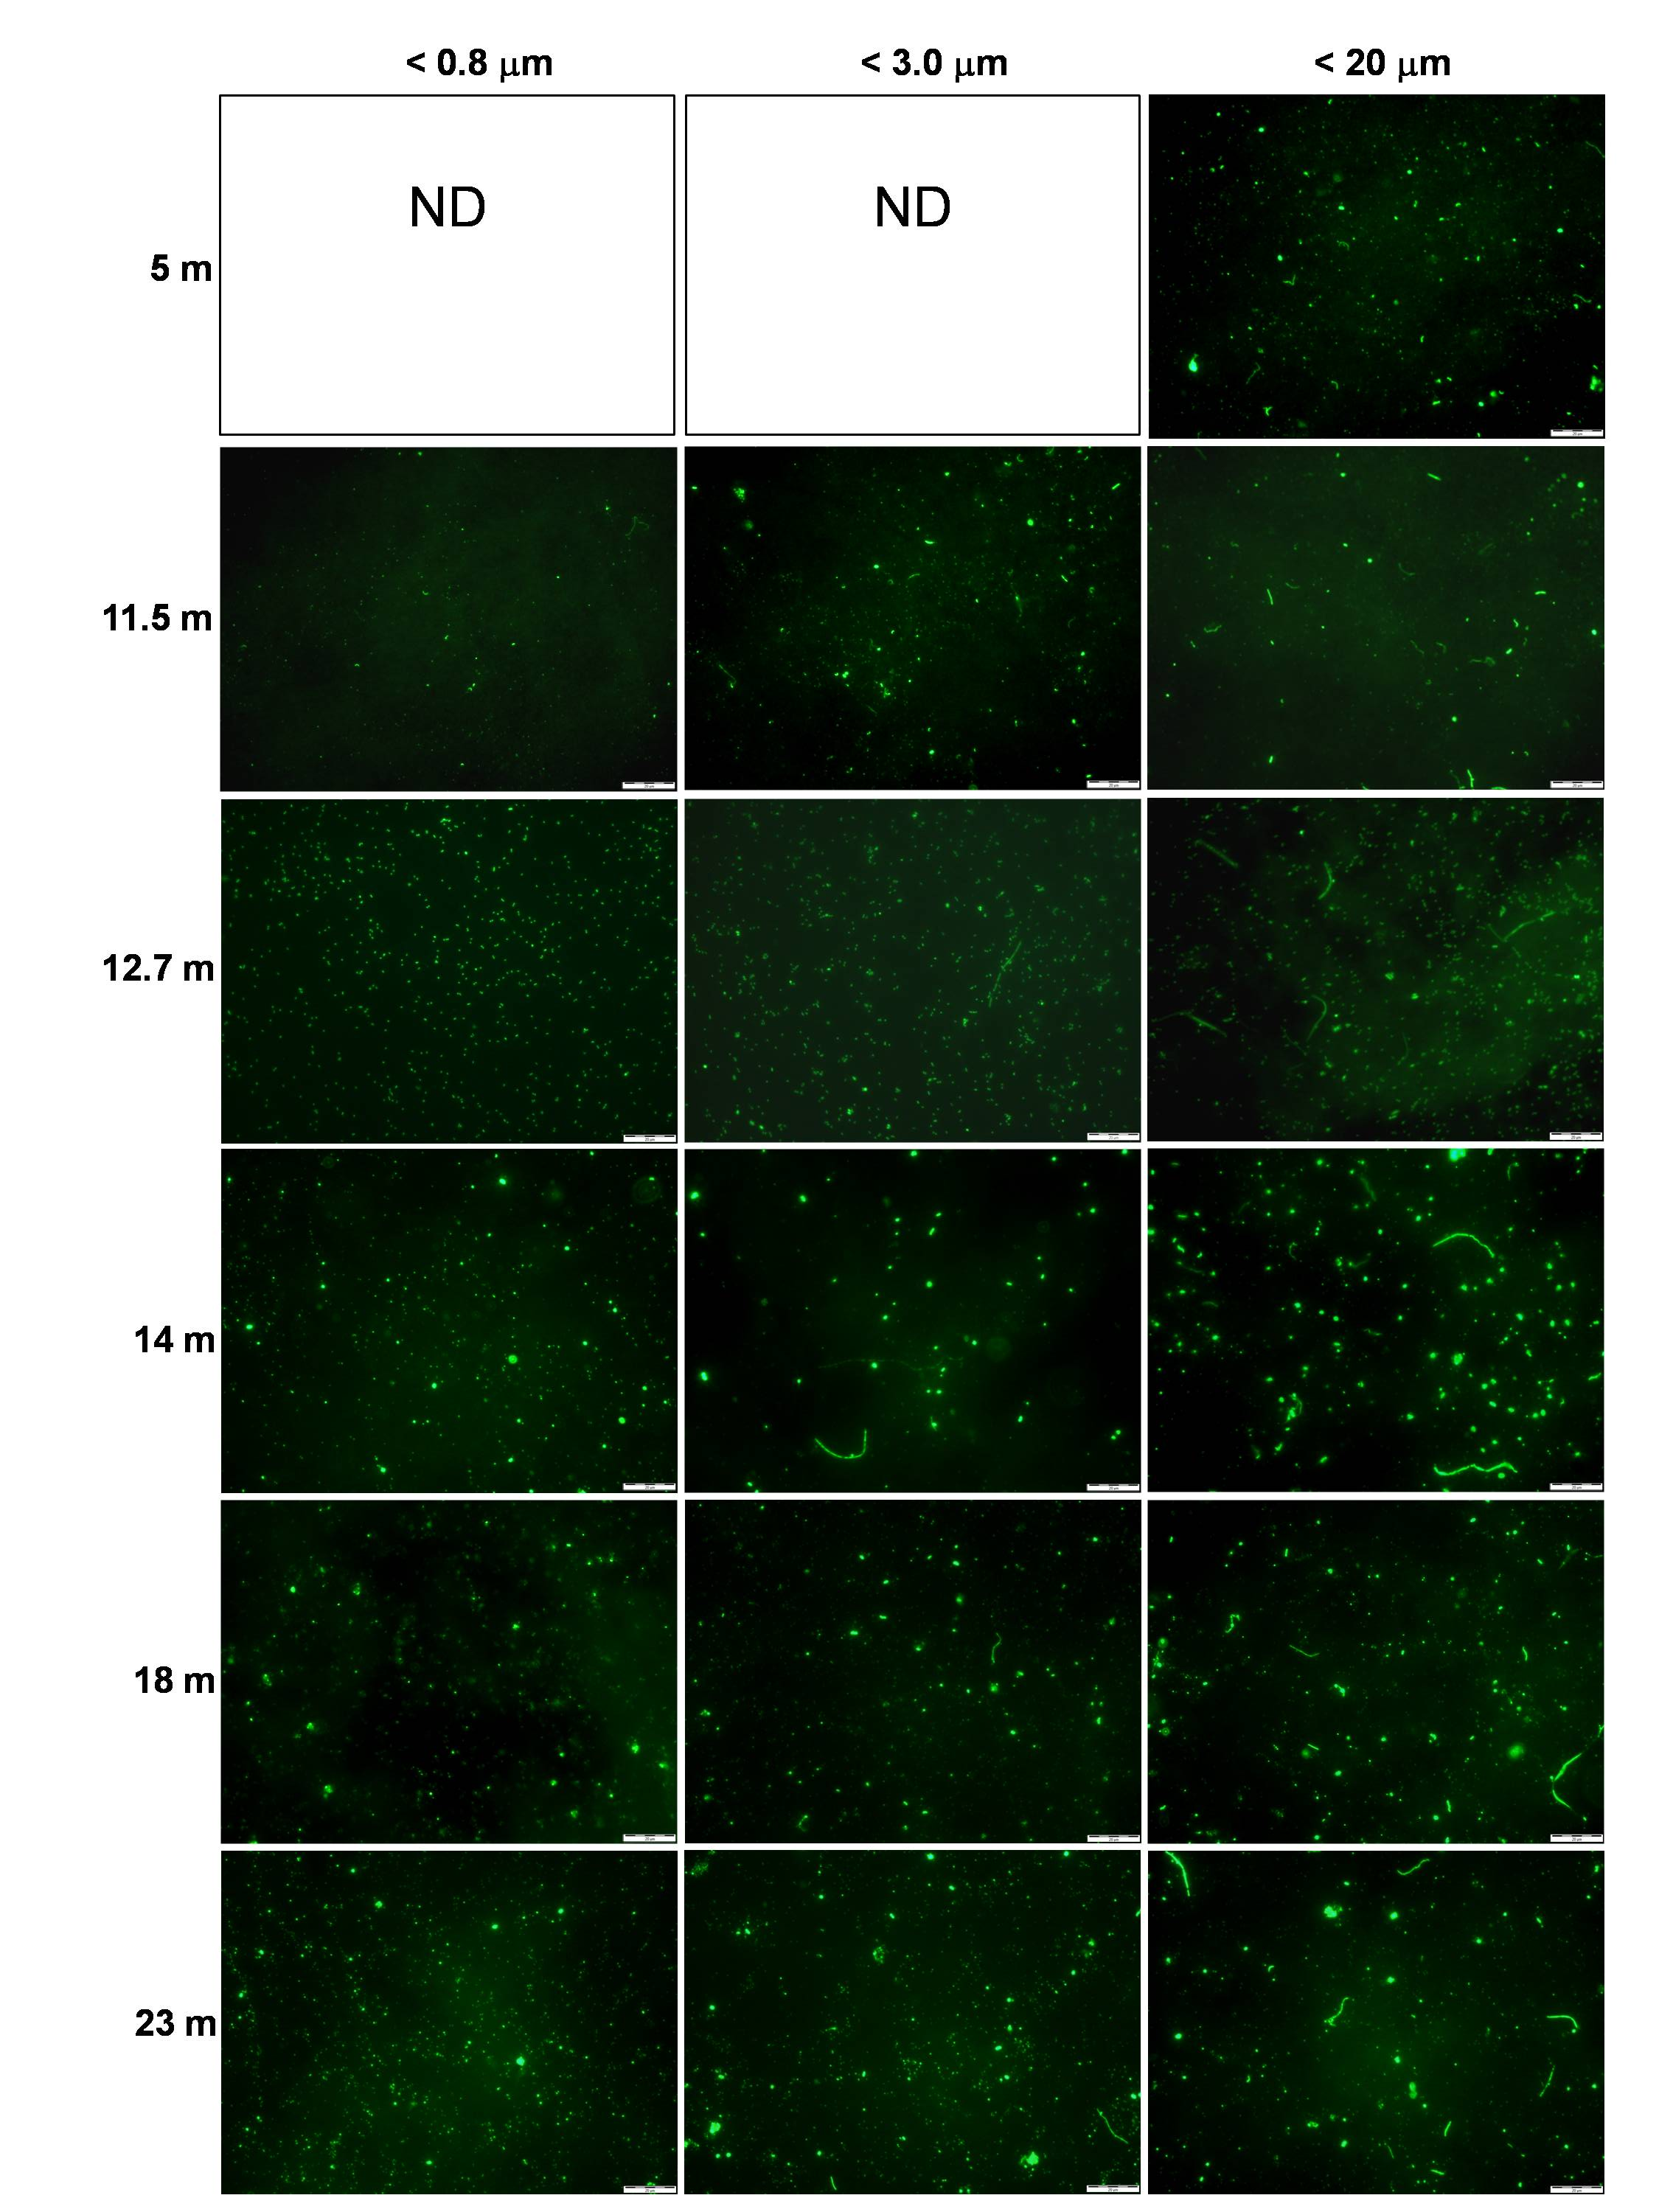
\includegraphics[width=\textwidth]{ace_figures/ace_microscopy.jpg}
\caption[Epifluorescence microscopy of Ace Lake microbiota]{Epifluorescence microscopy images of Ace Lake microbiota. Scale bar $=$ 20 \textmu{}m. ND, not determined.
}
\label{fig:ace_microscopy}

\end{figure}

To be competitive alternative to Anodisc filters in terms of accuracy of counts, a comparison of this methodolody and Anodisc-based protocols using viral samples of known densities needs to be performed.

\begin{figure}
\centering
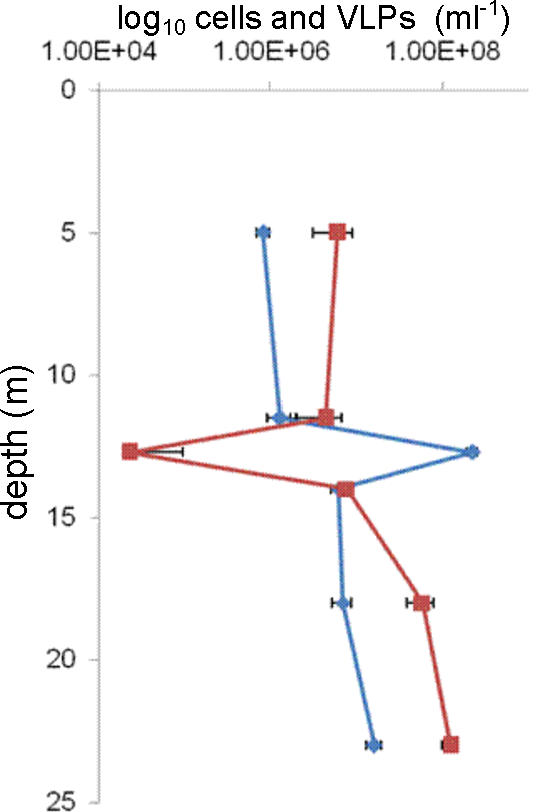
\includegraphics[width=50mm]{ace_figures/ace_counts.pdf}
\caption[Counts of microbial cells and \acs{VLP}s in Ace Lake]{Counts of microbial cells (blue) and \acs{VLP}s (red) by epifluorescence microscopy along a depth profile of Ace Lake.
Error bars represent one standard deviation.
No \acp{VLP} were detected at 12.7 m depth and the value reported represent the detection limit of the counting procedure (\emph{i.e.} one \acs{VLP} detected in one field of view).
}
\label{fig:ace_counts}

\end{figure}

No Anodisc filters could be obtained for such a comparative analysis to validate its use in this study.
However, for the purposes of this study, which is to show the relative differences in morphotypes between sample depths and size fractions, this method was more than suitable.
Other groups have since shown it to be comparable. %read papers and put in discussion.


\subsection[Community stratification supported by cell and \ac{VLP} densities]{Size and depth stratification of the community supported by cell and \ac{VLP} densities}
Development of fluorescence microscopy methodology using 0.01 \textmu{}m pore-size polycarbonate filters for simultaneous cellular and viral counts shows:

1. Size fractionation procedure appeared effective.

2. Morphological differences supports stratification of the community.

3. Visualisation of the morphology supported the metagenomic data that saw size fractionated and taxonomically stratified community.

4. Virus to bacteria ratios can give important information about the community.

At 12.7m depth, the light levels, and the sharp transition in oxygen content and salinity (Fig. S2) favour the dominance of a very high-density (2.2 $\times$ 10$^8$ cells ml$^{-1}$) of a single type of \ac{GSB} of the genus \emph{Chlorobia}, refered to as C-Ace \cite{Ng2010a}. 
Viral signatures were essentially devoid in this zone. 
The ratio of bacteriophage to total viral population increased proportionally in the larger size fractions consistent with trophic analyses that indicate that the larger size fractions are mostly copiotrophic (Fig. S8) particle attached bacteria and therefore likely to be sensitive to lysogenic phage infection \cite{Lauro2009}. 
The 23 m unfiltered lake water contained very high levels (1.3 $\times$ 10$^8$ \acp{VLP} ml$^{-1}$) of \acp{VLP}. 
The high diversity of bacteria and archaea in all size fractions of the monimolimnion (Fig. 2) is consistent with the presence of a high viral population (Rodriguez-Valera et al., NRM, 2009).


\subsection{Development of metaproteomic methodology}

1. Using a matched metagenome instead of \ac{NR} for protein identification greatly increased the number of identifications.
1.1 Except at the bottom zone, likely because the community is too diverse so greater coverage of the metagenome is required. %see available good spectra vs good reads
In parallel with taxonomic diversity increasing with depth (with the exception of the GSB layer), the rate of metaproteomic identification of proteins decreased with depth (Table S2). 
The majority of the proteins that were detected (e.g. 67\% at 23 m) were for hypothetical proteins that tended to lack orthologues in well-characterized organisms, highlighting both the functional importance and novelty of this anaerobic zone of the lake.


2. More specific information could be assigned to the taxonomic groups such as.
2.1. The Actinobacteria sequences in the mixolimnion were associated with a diverse phylogenetic cluster (Luna cluster) mainly contributed by freshwater ultramicrobacteria \cite{Hahn2003}. 
Several Luna cluster isolates contain rhodopsin genes \cite{Sharma2009} and similar gene sequences were present in the Ace Lake oxic zone data and found to be expressed (167820670 and 163154474; Table S2).
2.2.This is consistent with the identification of \ac{CRISPR} associated \ac{CAS} proteins Cse2, Cse3 and Cse4 (165526330, 165526332 and 165526334, respectively) in the 12.7 m metaproteome (Table S2). 
The \ac{CAS} gene locus (cas3, cse1, cse2, cse3, cse4, cas5, cas1b), to which the proteins map, shares its organisation with \ac{CAS} loci of sequenced \ac{GSB}, and groups with the \emph{E. coli} subtype/variant 2. The \ac{CRISPR}/\ac{CAS} system is likely to confer phage resistance to C-Ace, akin to the role in other organisms (Karginov and Hannon 2010; Horvath and Barrangou 2010).
%Recall that GSB all have large CRISPR regions and that the one in C-ace appears to be much reduced. Could this imply a lessening of viral load? The intervening spacers do not match to known viral sequences
% but did match to other GSB, could they be for competition?

3. Using \textsc{Scaffold} to validate protein identification and perform spectral counts was helpful. 
3.1Same protein identifications as Charmaine except one or two.
3.2 Able to quantify differences between mixolimnion and monimolimnion.
The diversity and abundance of \ac{ABC} transporters was lowest in the 0.1 \textmu{}m fractions at 23 m (Fig. 3), and a correspondingly low number were detected in the metaproteome (Table S2). 
In contrast, numerous transporters, predominately \ac{ABC} type, were identified in the metaproteome of the mixolimnion samples, with a high \ac{COG} representation of transporters for carbohydrates ($\sim$34\% of normalised spectra), amino acids ($\sim$32\%) and inorganic ions ($\sim$9\%) (Table S2 and Fig. S11).
All transporters in the metaproteome were of bacterial origin and conservative phylum level assignments of the normalised spectra showed the majority to originate from \emph{Proteobacteria} (69\%), 
of which SAR11 comprised 46\% and \emph{Actinobacteria} 19\% (Table S2). 
A high proportion of expressed genes with transport functions have also been reported for SAR11 from coastal (Poretsky et al. 2010) and open ocean waters (Sowell et al. 2009) (Morris et al. 2010?). 
Oligotrophs, such as SAR11 not only posses a low-diversity of high-affinity transporters (Lauro et al., 2009), but regulate the relative abundance of transporters expressed in response to \ac{DOC} availability (Poretsky et al. 2010). 
The prevalence of amino acid and simple sugar transporters (Table S2), and the low \ac{DOC} concentration in the Ace Lake mixolimnion (Fig. 1) is likely to reflect efficient utilisation of these substrates from the \ac{DOC} pool. 
Two SAR11 transport proteins that were detected in Ace Lake (Table S2) were not detected from the Sargasso Sea (Sowell,et al. 2009): an ectoine/hydroxyectoine (167807477 and 167892279) and a zinc \ac{ABC} transporter (167933120). The zinc \ac{ABC} transporter is likely to support zinc efflux in response to zinc concentrations which are $\sim$70-fold higher in the mixolimnion of Ace Lake compared to seawater (Rankin 1999). 
Conversely, phosphate transporters were a major class detected from the Sargasso Sea (Sowell,et al. 2009) but were absent from the Ace Lake metaproteome; consistent with lower phosphate levels in the Sargasso Sea ($<$5 nM) compared to Ace Lake (1--12 \textmu{}M). The differences in transporter expression between Ace Lake and oceanic SAR11 are likely to signify adaptive growth strategies that have evolved in the Ace Lake SAR11 community.
The high numbers of bacteriophages in the monimolimnion (detected by microscopy, Fig. S5 and S6; metaproteomics, Table S2; metagenomics, Fig. 2), and increase in \ac{DOC} observed at depth (Fig. 1), also indicates that carbon turnover in the monimolimnion is likely to be tightly coupled to the carbon flux going through a viral shunt, as proposed for open ocean systems (Suttle, C. A. Viruses in the sea. Nature 437, 356–361 (2005)). 
The bacteriophages are also likely vehicles for mediating gene exchange.
Most of the genetic potential to cycle the nitrogen pool appears to be limited to nitrogen assimilation throughout the lake and remineralisation in the monimolimnion (Fig. S14). 
The detection of glutamine synthetase (GlnA) and glutamate synthases (GltBS) in the metaproteome (Table S2) are supportive of active nitrogen assimilation. 
In the mixolimnion, GlnA was linked to SAR11 and \emph{Actinobacteria}, and they are likely to be responsible for nitrogen absorption in the oxic zone. At the oxycline, GlnA and GltB from GSB were abundant (Table S2), indicating an important role for nitrogen assimilation at this zone in the lake.
Genes for \ac{ASR} were present in metagenome data of all three fractions at all depths, although they were lowest at the oxycline. 
However, there was no evidence for expression of the genes as ASR proteins were not detected by metaproteomics. In contrast, multiple subunits of the GSB dissimilatory sulfide reductase complex were identified (Ng et al. 2010 and Table S2) indicating functionality of this pathway at the oxycline. 
\ac{GSB} likely utilise the dissimilatory sulfide reductase system to convert sulphur to sulfite and the polysulfide-reductase-like complex 3 to oxidize sulfite to sulphate. 
SRB may then reform sulphide completing the sulphur cycle between the \ac{GSB} and \ac{SRB} (Ng et al. 2010). 
While \ac{SRB} were detected at the three depths of the monimolimnion, sulphate is depleted in the water column and sediment at the bottom of the lake limiting their dissimilatory capacity \cite{Rankin1999}. 
Finally, sulphate in the mixolimnion can be linked to sulphur-oxidation by SAR11 (Meyer and Kuever, Microbiology 153:3478-3498) and a concomitant lack of capacity to perform sulphur reduction. 


%--------------------------------------------------------------------------------------------
\section{Conclusions}
Using complementary approaches helps to validate the research methodology and 
metagenomic inferences about the whole community.
Specifically, differences in size and depth was shown by both microscopy and metagenomics to be apparent.
This both validates the method of size fractionation as a viable approach to broad separation of the community,
as well as supports the assertion that there was a large difference in community at different depths.
Using a matched metaproteomic database showed a huge increase in the number of protein identifications.
This was provided that metagenomic coverage was good.
Using a metaproteomics, genes identified as potentially relevant in the metagenome were found to be expressed, supporting their importance.
For example, it showed the \ac{CRISPR} genes were active and may be a defence against phage.
It also showed Actinorhodopsins were expressed.
It showed that abundant genes were normally abundant in the metaproteome, such as transport proteins that give insight into what substrates are important components of the \ac{DOC} pool.
New inferences could be drawn from the metaproteome, such as the preference for labile substrates such as active sulfate reduction which is not apparent from the sulphate concentration.



%--------------------------------------------------------------------------------------------
